\clearpage
\section{Do Winners Contest the Next Election?}\label{sec:recontesting}
\suppressfloats[t]

One way quotas could increase women's subsequent representation is by helping the women elected under them build continuing political careers. We examine this route by linking Rajasthan's 2015 winners to candidates in 2020 and Uttar Pradesh's 2015 winners to candidates in 2021. This differs from the aggregate candidacy analysis in Appendix~\ref{sec:app_outcomes}: the outcome here concerns the previous winner, rather than all women who enter the next election.

\subsection{Data and matching}

We use the State Election Commission winner and candidate records and the GP links described in Appendix~\ref{sec:app_data}. We restrict the follow-up election to seats reserved for neither women nor a caste group, so the new reservation category does not bar any prior winner from contesting. The comparison includes all prior non-quota winners, including women. Rajasthan's candidate rosters must contain the number of contestants reported in the official results and refer to a unique election event. UP's rosters must contain a single declared winner consistent with the linked panel; an independent contestant count is unavailable. Table~\ref{tab:recontesting_coverage} reports coverage.

\begin{table}[!htbp]
\centering
\caption{Coverage of the Winner-to-Candidate Comparison}
\label{tab:recontesting_coverage}
\small
\begin{tabular}{llrrrr}
\toprule
Cohort & Prior seat & Linked & Fully open & Roster checks & Analysis \\
\midrule
Rajasthan & Quota & 3821 & 1202 & 1196 & 1195 \\
Rajasthan & Non-quota & 4061 & 707 & 705 & 704 \\
Uttar Pradesh & Quota & 15621 & 9918 & 9917 & 9803 \\
Uttar Pradesh & Non-quota & 30893 & 6561 & 6561 & 6461 \\
\bottomrule
\end{tabular}

\begin{minipage}{\textwidth}\footnotesize
\emph{Notes:} Rajasthan follows 2015 winners to 2020; UP follows 2015 winners to 2021. ``Fully open'' means no gender or caste reservation at follow-up. Roster checks require nonmissing candidate names, unique candidate identifiers, and the state-specific checks described in the text. The analysis also requires usable prior-winner identifiers and excludes ambiguous exact matches or exact matches conflicting with recorded sex or feasible age. All matching rules use the same sample within each state.
\end{minipage}
\end{table}

There is no common person identifier across elections. Our strict rule requires a unique normalized name match within the linked GP; in UP it also requires the recorded father's or husband's name to match. We normalize case, punctuation, and whitespace while retaining Hindi vowel signs. For more generous matching, we transliterate names into Latin script and remove spaces. A candidate's name may then differ by up to two character edits and no more than 20\% of the longer name; nonexact matches require both names to contain at least five characters. UP also has an intermediate rule requiring the relative's name to agree within three edits and 25\%. The most generous rule allows a compatible candidate-name match without requiring agreement on the relative's name, and counts any such candidate as a possible return.

Recorded sex must be compatible. We also reject matches to candidates younger than 25 in Rajasthan or 26 in UP at follow-up, ages inconsistent with having reached 21 in 2015 after allowing for election dates within each year (Constitution of India, Article~243F). Prior-winner age is unavailable, so age cannot otherwise verify identity; missing follow-up age remains unknown. These rules address spelling and recording differences without treating every similar name as a verified identity. Strict matching can miss genuine returns, while generous matching can admit namesakes. The resulting rates describe matching scenarios, not formal bounds on the true rate of contesting again.

\subsection{Results}

Under strict matching, \recontestRajQuotaRate{}\% of Rajasthan's prior quota winners reappear in the next candidate roster, compared with \recontestRajNonquotaRate{}\% of prior non-quota winners. The corresponding UP rates are \recontestUpQuotaRate{}\% and \recontestUpNonquotaRate{}\%. Adjusting for baseline block and caste reservation gives differences of \recontestRajDifference{} percentage points in Rajasthan (95\% interval [\recontestRajLow{}, \recontestRajHigh{}]) and \recontestUpDifference{} points in UP ([\recontestUpLow{}, \recontestUpHigh{}]). These are comparisons between the officeholders selected under the two reservation regimes, not estimates of the effect of winning office on the same person's subsequent career.

\begin{table}[!htbp]
\centering
\caption{Prior Winners Matched to Candidates in the Next Election}
\label{tab:recontesting}
\small
\begin{tabular}{lrrrr}
\toprule
 & \multicolumn{2}{c}{Matched / prior winners (\%)} & \multicolumn{2}{c}{Adjusted difference (pp)} \\
Cohort & Quota & Non-quota & Estimate & 95\% interval \\
\midrule
Rajasthan & 34/1195 (2.8) & 95/704 (13.5) & -11.5 & [-14.6, -8.3] \\
Uttar Pradesh & 983/9803 (10.0) & 1069/6461 (16.5) & -5.7 & [-6.9, -4.6] \\
\bottomrule
\end{tabular}

\begin{minipage}{\textwidth}\footnotesize
\emph{Notes:} Strict matching in seats fully open at follow-up. Counts and percentages are unadjusted. Adjusted differences are quota minus non-quota coefficients from linear probability models with baseline block fixed effects and baseline caste-reservation indicators. The samples contain \recontestRajClusters{} blocks in Rajasthan and \recontestUpClusters{} in UP. Intervals use block-clustered standard errors, the manuscript's finite-sample correction, and a cluster-$t$ reference distribution. They describe sampling uncertainty conditional on the matching rule, not uncertainty about identities.
\end{minipage}
\end{table}

Generous matching raises the rates to \recontestRajGenerousQuotaRate{}\% versus \recontestRajGenerousNonquotaRate{}\% in Rajasthan and \recontestUpGenerousQuotaRate{}\% versus \recontestUpGenerousNonquotaRate{}\% in UP. Requiring a similar relative's name in UP gives intermediate rates of \recontestUpFuzzyQuotaRate{}\% and \recontestUpFuzzyNonquotaRate{}\%. Thus the levels depend substantially on how identities are matched, but prior quota winners are less likely to appear under every rule (Figure~\ref{fig:recontesting}). The comparison is consistent with limited continuation by the original quota winners. It does not exclude entry by other women, candidacy in another GP or office, or differences in matching accuracy between quota and non-quota winners.

Low rates of return also appear in earlier evidence: the 2008 Panchayati Raj Ministry report finds that over 89\% of women representatives did not contest another election after their term \citep[pp.~26, 63]{ministry2008}.

\begin{figure}[!htbp]
\centering
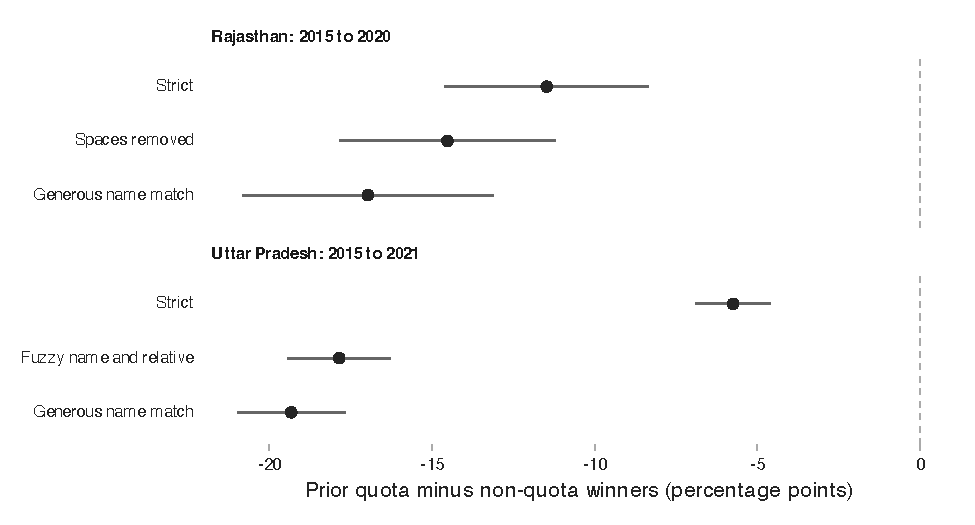
\includegraphics[width=\textwidth]{../figs/recontesting.pdf}
\caption{Sensitivity of Subsequent Candidacy Comparisons to Matching Rules}
\label{fig:recontesting}
\begin{minipage}{\textwidth}\footnotesize
\emph{Notes:} Points are adjusted differences in matched candidacy between prior quota and non-quota winners, in percentage points; lines are 95\% block-clustered intervals. Each state uses a common sample across rules. Strict matching requires the name in Rajasthan and both name and relative in UP. The other rules remove spaces or allow the transliteration and edit-distance matches described in the text. The generous rule counts any compatible candidate-name match as a possible return. Zero denotes no difference. Intervals do not incorporate linkage uncertainty.
\end{minipage}
\end{figure}
\FloatBarrier
